{
Det vi kalder det gyldne snit, den gyldne ratio eller det guddommelige
forhold, blev allerede beskrevet i Euklids \emph{Elements} fra ca. 300
f.  Kr. som følger:
\begin{quote}
	\emph{``A straight line is said to have been cut in extreme
	and mean ratio when, as the whole line is to the greater
	segment, so is the greater to the less.''}\cite{Euclid300bc}
\end{quote}

\begin{figure}[h!]
	\begin{center}
		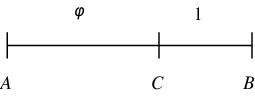
\includegraphics[scale=0.49,angle=0]{afsnit/baggrund/billeder/line_segment_a_c_b}
	\end{center}
	\caption{Euklids opdeling af et linjestykke}
	\label{line_segment}
\end{figure}

Givet et linjestykke $A\ B$, hvor $A\ B$ definerer linjen mellem
punkterne $A$ og $B$, som vist i figur \ref{euclid}, og ud fra Euklids
beskrivelse kan $\varphi$ defineres som
\begin{equation}
	\varphi	= \frac{A\ C}{C\ B} = \frac{A\ B}{A\ C}
	\label{euclid}
\end{equation}
Ved at indsætte variable i ligning \ref{euclid} får vi
\begin{equation}
	\varphi = \frac{\varphi + 1}{\varphi}
	\label{expand_euclid}
\end{equation}
hvilket giver os andengradsligningen
\begin{equation}
	\varphi^{2} - \varphi - 1 = 0.
	\label{poly_phi}
\end{equation}
Hvis vi nu løser andengradsligningen i \ref{poly_phi}, med
$\varphi > 0$, får vi
\begin{eqnarray*}
	\varphi	& =	& \frac{\sqrt{5} + 1}{2} \\
		& =	& 1.6180\ 3398\ 8749\ 8948\ 4820 \dots
\end{eqnarray*}

Tallet $\varphi$ bemærker sig blandt andet ved, at når det kvadreres, så
lægger man blot 1 til. Dette udledes trivielt fra ligning \ref{poly_phi}
\begin{equation}
	\varphi^{2} = \varphi + 1
	\label{phi_squared}
\end{equation}

Vi kan også finde polynomiets anden rod som angives ved $\varPhi$
\begin{eqnarray*}
	\varPhi & = & \frac{1}{\varphi} \\
		& = & \varphi - 1 \\
		& = & 0.6180\ 3398\ 8749\ 8948\ 4820 \dots
\end{eqnarray*}
Også tallet $\varPhi$ er interessant idet dets eget kvadrat plus sig
selv giver 1. Vi har at
\begin{equation}
	\varPhi^{2} + \varPhi = 1
	\label{Phi_squared}
\end{equation}
hvilket kun er gældende for $\varPhi$.

Det gyldne snit fremviser endvidere en interessant forbindelse til
Fibonaccis talrække, da forholdet mellem to fibonaccital $F(n)$ og $F(n
- 1)$ konvergerer mod $\varphi$ når $n$ nærmer sig uendelig. Formelt har
vi at
\begin{eqnarray*}
	\varphi & =     & \lim_{n \rightarrow\infty}{\frac{F(n)}{F(n - 1)}}
\end{eqnarray*}

I tabel \ref{fibonacci_sequence} kan ses hvordan ratioen mellem
fibonaccital konvergerer mod $\varphi$, hvor vi også viser den
procentvise afvigelse fra $\varphi$.

\begin{table}[h!]
    \centering
    \begin{tabular}{|c|c|c|c|c|}
        \hline
        $n$ & $F(n)$ & $F(n - 1)$ & $ \frac{F(n)}{F(n - 1)}$ & $\%$ fra $\varphi$ \\
        \hline
        0	 & 0 	 & $n/a$ & $n/a$ 		& $n/a$ 		\\
        1	 & 1	 & 1	 & 1.0		 	& 38.196601125 		\\
        2	 & 1	 & 1	 & 1.0		 	& 38.196601125 		\\
        3	 & 2	 & 1	 & 2.0		 	& -23.60679775 		\\
        4	 & 3	 & 2	 & 1.5			& 7.29490168752 	\\
        5	 & 5	 & 3	 & 1.66666666667	& -3.00566479165 	\\
        6	 & 8	 & 5	 & 1.6			& 1.11456180002 	\\
        7	 & 13	 & 8	 & 1.625	 	& -0.430523171858 	\\
        8	 & 21	 & 13	 & 1.61538461538	& 0.163740278863 	\\
        9	 & 34	 & 21	 & 1.61904761905	& -0.062645797602 	\\
        10	 & 55	 & 34	 & 1.61764705882	& 0.0239135845758 	\\
        11	 & 89	 & 55	 & 1.61818181818	& -0.00913636134662 	\\
        12	 & 144	 & 89	 & 1.61797752809	& 0.00348946069118 	\\
        13	 & 233	 & 144	 & 1.61805555556	& -0.00133290189271 	\\
        \hline
    \end{tabular}
    \caption{Fibonaccisekvens}
    \label{fibonacci_sequence}
\end{table}

\subsection{Et gyldent rektangel}
På samme måde som vi kan opdele en linjestykke efter det gyldne snit,
kan vi konstruere et rektangel hvor forholdene mellem højde og bredde er
$\varphi$. Vi konstruerer et rektangel hvor alle sider er lig 1 og
tegner en diagonal fra dette rektangelels midte til modsatte hjørne. Med
denne diagonal som radius tegnes en cirkel som et gyldent rektangel kan
tegnes efter. Figur \ref{golden_rectangle} illustrerer denne metode.

\begin{figure}[h!]
	\begin{center}
		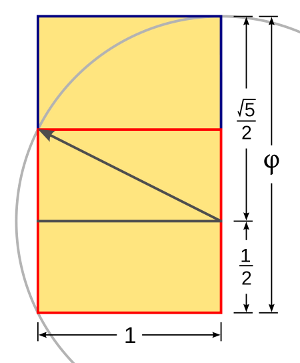
\includegraphics[scale=0.35,angle=0]{afsnit/baggrund/billeder/Golden_Rectangle_Construction}
	\end{center}
	\caption[Et gyldent rektangel]{Et gyldent rektangel - \emph{Kilde: Wikipedia}}
	\label{golden_rectangle}
\end{figure}
Det ses at rektanglet har forholdet $\varphi:1$ og at eksemplet er helt
analogt til det linjestykke givet i figur \ref{line_segment}. Dog skal
det bemærkes, at det rektangel der kan konstrueres af linjestykkerne 1
og $\varphi - 1$ også er et gyldent rektangel med forholdet $1:\varphi
-1 = \varphi$. Man kan derved konstruere gyldne rektangler ud i det
uendelige ved hele tiden at lave nye gyldne rektangler.

\subsection{Spiraler og det gyldne snit}
Når man som ovenfor, gentagende gange deler et gyldent rektangel kan man
bruge dette til at konstruere en gylden spiral. En gylden spiral kan
skrives ved ligningen for generelle logaritmiske spiraler som
\begin{equation}
	r = ae^{c\theta}
	\label{log_spiral_2}
\end{equation}
eller
\begin{equation}
	\theta = \frac{1}{c}\ln(r/a)
	\label{log_spiral_1}
\end{equation}
hvor $e$ er grundtallet for den naturlige logaritme og $c$ skal have en
speciel værdi for at kunne være en gylden spiral. Den gyldne spiral kan

Det kan være svært at tegne logaritmiske spiraler korrekt, men man kan
approksimere en spiral ved at sammensætte dele af cirkler. Derved kan
man approksimere en gylden spiral ved at sammensætte kvarte cirkler.
Denne approksimation giver dog ikke en ægte gylden spiral og faktisk kan
ingen sådanne approksimationer af sammensatte cirkler gengives ved en
matematisk ligning\cite{Sharp2002}. Det er i tabel
\ref{fibonacci_sequence} vist hvordan Fibonaccis talrække konvergerer
mod det gyldne snit. Vi kan også konstruere et approksimeret gyldent
rektangel ud fra fibonaccitallene, som vist i figur
\ref{fibonacci_rektangel}, ved sammensatte $F(n)$ x $F(n)$-rektangler.
\begin{figure}[h!]
	\begin{center}
		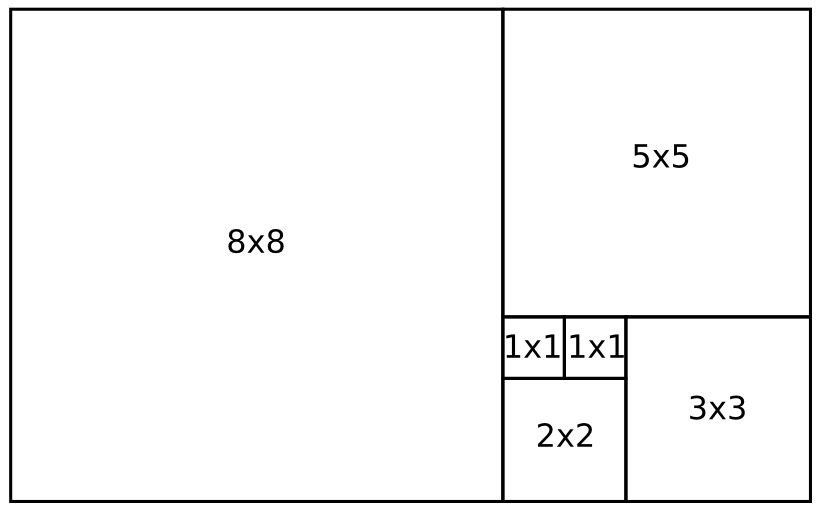
\includegraphics[scale=0.35,angle=0]{afsnit/baggrund/billeder/fib_rect}
	\end{center}
	\caption[Rektangel opbygget efter Fibonaccis talrække]{Rektangel
	opbygget efter Fibonaccis talrække. Man kan blive ved med at
	sætte $F(n)$ x $F(n)$-rektangler på denne figur og kan derved
	nærme sig et ægte gyldent rektangel jvf. tabel
	\ref{fibonacci_sequence}.}
	\label{fibonacci_rektangel}
\end{figure}
Vi kan nu tegne kvarte cirkler i figur \ref{fibonacci_rektangel} med
radius $F(n)$ og derved approksimere en gylden spiral som vist i figur
\ref{fibonacci_spiral}. Hvor tæt vi kommer på en egentlig gylden spiral
afhænger af hvor mange rektangler vi har brugt til at tegne spiralen
efter. Et højere antal rektangler giver en spiral som et tættere på en
egentlig gylden spiral. Formelt kan det direkte udledes af tabel
\ref{fibonacci_sequence} hvor tæt en approksimation vi har på en gylden
spiral.
\begin{figure}[h!]
	\begin{center}
		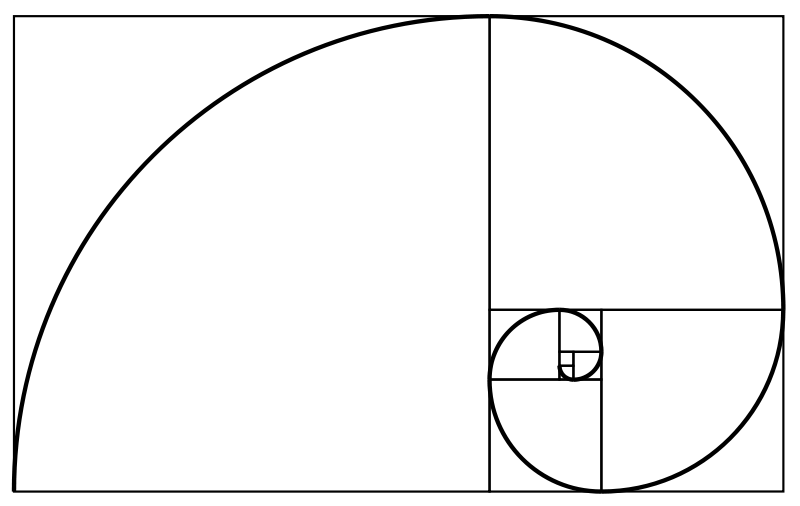
\includegraphics[scale=0.35,angle=0]{afsnit/baggrund/billeder/Fibonacci_spiral}
	\end{center}
	\caption[En fibonaccispiral]{En fibonaccispiral - \emph{Kilde: Wikipedia}}
	\label{fibonacci_spiral}
\end{figure}
Hvis man regner den korrekte faktor $c$ ud og tegner en ægte gylden
spiral i et gyldent rektangel vil man se at spiralen faktisk går
\emph{udenfor} rektanglet\cite{Sharp2002}. Ovenstående approksimation
med radius $F(n)$ vil aldrig gå udover rektanglet og det bliver derved
klart at fibonaccispiralen i sandhed blot er en approksimation.

For en fuld gennemgang af spiraler, specielt med henblik på det gyldne
snit, se \cite{Sharp2002}. Vi vil nu kaste et hurtigt blik på
problematikken ved at afgøre hvad der er interessant i et billede og se
på hvordan computeren kan bruges i denne sammenhæng.

}
% vim: set tw=72 spell spelllang=da:
